\section{Application to the Example and Discussion}
\label{sec:discussion}

    This section proposes to illustrate the proposed transformation from AAF to action language for Example~\ref{ex:IRM_ou_radio}, highlighting its exploitation to get enriched information about the modelled dialogue, more precisely for providing visual representations justifying the acceptance or rejection of arguments. It considers successively two classes of argumentation explanations in \cite{cyras_survey}'s taxonomy: 
    it first shows how it can lead to graphical representations of the processes of accepting/rejecting arguments, it then discusses the case of causal explanations. 


        %In this section we apply program~$\Pi(\chi)$ to Example~\ref{ex:IRM_ou_radio}. The event trace $\tau_{\chi}^e$ and state trace~$\tau_{\chi}^s$, as well as the causal relations lead to Figures~\ref{fig:exemple_ini} and~\ref{fig:exemple_fin}.
        
    \subsection{Graphical Representation and Explanation}
    \label{sec:discu_temps}

    According to \cite{cyras_survey}, argumentation explanations can consist in extracting argumentative subgraphs to justify the acceptance or rejection of an argument for a given AAF semantics, producing a graphical representation of the underlying process.

% In argumentation, \cite{cyras_survey} proposed a classification of methods for generating explanations. Among them, one category focuses on the extraction of argumentative subgraphs to justify the acceptance or rejection of an argument for a certain semantics, producing a graphical representation of the process of accepting or rejecting an argument.
        
The transformation proposed in the previous section makes it possible to derive  graphical representations of the argumentative process. Indeed, the traces of events and states can be used  to obtain a narrative of the interaction that can be represented graphically. The visualisation we propose is illustrated in Figure~\ref{fig:exemple_ini}, in a simplified form, for Example~\ref{ex:IRM_ou_radio}. It is enriched in the next section using causality relations.


        \begin{figure}[t]
            \centering
        	\resizebox{7cm}{!}{

\tikzset{every picture/.style={line width=0.75pt}} %set default line width to 0.75pt        

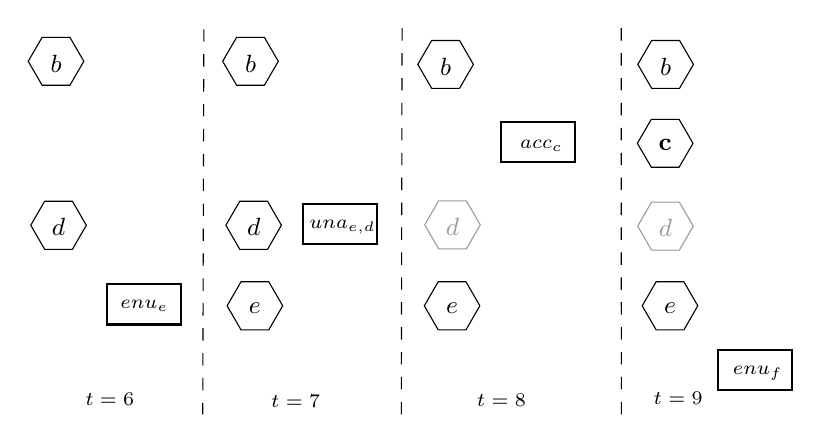
\begin{tikzpicture}[x=0.75pt,y=0.75pt,yscale=-1,xscale=1]
%uncomment if require: \path (0,300); %set diagram left start at 0, and has height of 300

%Shape: Rectangle [id:dp32394197299921523] 
\draw  [line width=0.75]  (38.8,129.2) -- (74.6,129.2) -- (74.6,148.54) -- (38.8,148.54) -- cycle ;
%Straight Lines [id:da5103454315814933] 
\draw  [dash pattern={on 4.5pt off 4.5pt}]  (85.53,6.3) -- (85,191.83) ;
%Straight Lines [id:da9625799604219181] 
\draw  [dash pattern={on 4.5pt off 4.5pt}]  (181.03,5.8) -- (180.67,191.83) ;
%Straight Lines [id:da937826652519754] 
\draw  [dash pattern={on 4.5pt off 4.5pt}]  (286.6,5.8) -- (286.67,191.83) ;
%Shape: Rectangle [id:dp39055029505322625] 
\draw  [line width=0.75]  (133.09,90.57) -- (168.89,90.57) -- (168.89,109.91) -- (133.09,109.91) -- cycle ;
%Shape: Polygon [id:dp25831662543105294] 
\draw   (27.7,21.73) -- (21,33.26) -- (7.6,33.26) -- (0.91,21.73) -- (7.6,10.19) -- (21,10.19) -- cycle ;
%Shape: Polygon [id:dp17264867524000027] 
\draw   (121.4,21.73) -- (114.7,33.26) -- (101.3,33.26) -- (94.6,21.73) -- (101.3,10.19) -- (114.7,10.19) -- cycle ;
%Shape: Polygon [id:dp9933858680624272] 
\draw   (215.4,23.23) -- (208.7,34.76) -- (195.3,34.76) -- (188.6,23.23) -- (195.3,11.69) -- (208.7,11.69) -- cycle ;
%Shape: Polygon [id:dp7138531738923998] 
\draw   (321.2,61.23) -- (314.5,72.76) -- (301.1,72.76) -- (294.4,61.23) -- (301.1,49.69) -- (314.5,49.69) -- cycle ;
%Shape: Regular Polygon [id:dp10291797427860683] 
\draw   (323.5,139.53) -- (316.81,151.12) -- (303.43,151.12) -- (296.74,139.53) -- (303.43,127.95) -- (316.81,127.95) -- cycle ;
%Shape: Regular Polygon [id:dp2894654570081998] 
\draw   (218.5,139.53) -- (211.81,151.12) -- (198.43,151.12) -- (191.74,139.53) -- (198.43,127.95) -- (211.81,127.95) -- cycle ;
%Shape: Regular Polygon [id:dp8293769486214224] 
\draw   (122.9,100.73) -- (116.21,112.32) -- (102.83,112.32) -- (96.14,100.73) -- (102.83,89.15) -- (116.21,89.15) -- cycle ;
%Shape: Regular Polygon [id:dp8361683320569804] 
\draw   (123.5,139.53) -- (116.81,151.12) -- (103.43,151.12) -- (96.74,139.53) -- (103.43,127.95) -- (116.81,127.95) -- cycle ;
%Shape: Regular Polygon [id:dp5470998290634859] 
\draw   (28.9,100.73) -- (22.21,112.32) -- (8.83,112.32) -- (2.14,100.73) -- (8.83,89.15) -- (22.21,89.15) -- cycle ;
%Shape: Rectangle [id:dp8416513794122603] 
\draw  [line width=0.75]  (228.69,50.97) -- (264.49,50.97) -- (264.49,70.31) -- (228.69,70.31) -- cycle ;
%Shape: Rectangle [id:dp842481801930145] 
\draw  [line width=0.75]  (333.09,160.97) -- (368.89,160.97) -- (368.89,180.31) -- (333.09,180.31) -- cycle ;
%Shape: Regular Polygon [id:dp0962459706720944] 
\draw  [color={rgb, 255:red, 155; green, 155; blue, 155 }  ,draw opacity=1 ] (218.7,100.53) -- (212.01,112.12) -- (198.63,112.12) -- (191.94,100.53) -- (198.63,88.95) -- (212.01,88.95) -- cycle ;
%Shape: Regular Polygon [id:dp5093510894708538] 
\draw  [color={rgb, 255:red, 155; green, 155; blue, 155 }  ,draw opacity=1 ] (321.3,101.13) -- (314.61,112.72) -- (301.23,112.72) -- (294.54,101.13) -- (301.23,89.55) -- (314.61,89.55) -- cycle ;
%Shape: Polygon [id:dp3364030899411299] 
\draw   (321.4,23.23) -- (314.7,34.76) -- (301.3,34.76) -- (294.6,23.23) -- (301.3,11.69) -- (314.7,11.69) -- cycle ;

% Text Node
\draw (27.13,180.4) node [anchor=north west][inner sep=0.75pt]  [font=\scriptsize]  {$t=6$};
% Text Node
\draw (44,135.6) node [anchor=north west][inner sep=0.75pt]  [font=\scriptsize]  {$enu_{e}$};
% Text Node
\draw (135.09,96.97) node [anchor=north west][inner sep=0.75pt]  [font=\scriptsize]  {$una_{e,d}$};
% Text Node
\draw (116.67,181.33) node [anchor=north west][inner sep=0.75pt]  [font=\scriptsize]  {$t=7$};
% Text Node
\draw (215.8,180.9) node [anchor=north west][inner sep=0.75pt]  [font=\scriptsize]  {$t=8$};
% Text Node
\draw (301,179.9) node [anchor=north west][inner sep=0.75pt]  [font=\scriptsize]  {$t=9$};
% Text Node
\draw (14.3,22.73) node  [font=\small]  {$b$};
% Text Node
\draw (108,22.73) node  [font=\small]  {$b$};
% Text Node
\draw (202,24.23) node  [font=\small]  {$b$};
% Text Node
\draw (307.8,62.23) node  [font=\small]  {$\mathbf{c}$};
% Text Node
\draw (310.12,140.53) node  [font=\small]  {$e$};
% Text Node
\draw (205.12,140.53) node  [font=\small]  {$e$};
% Text Node
\draw (109.52,101.73) node  [font=\small]  {$d$};
% Text Node
\draw (110.12,140.53) node  [font=\small]  {$e$};
% Text Node
\draw (15.52,101.73) node  [font=\small]  {$d$};
% Text Node
\draw (236.69,58.57) node [anchor=north west][inner sep=0.75pt]  [font=\scriptsize]  {$acc_{c}$};
% Text Node
\draw (339.09,167.57) node [anchor=north west][inner sep=0.75pt]  [font=\scriptsize]  {$enu_{f}$};
% Text Node
\draw (205.32,101.53) node  [font=\small,color={rgb, 255:red, 155; green, 155; blue, 155 }  ,opacity=1 ]  {$d$};
% Text Node
\draw (307.92,102.13) node  [font=\small,color={rgb, 255:red, 155; green, 155; blue, 155 }  ,opacity=1 ]  {$d$};
% Text Node
\draw (308,24.23) node  [font=\small]  {$b$};


\end{tikzpicture}
}
        	\caption{Partial graphical representation 
        	%of event and state traces $\tau_{\chi}^e$ and $\tau_{\chi}^s$ 
        	associated to Example~\ref{ex:IRM_ou_radio}. 
        	Hexagons represent fluents and rectangles events.
        	}
        	\label{fig:exemple_ini} 
        \end{figure}

        \begin{table}[t]
        \footnotesize
        \addtolength{\tabcolsep}{-1pt}
        \begin{center}
            \begin{tabular}{|c|cccccccccccc|c|}
        % \hline
        %  & \multicolumn{13}{c|}{Séquence d'action $enunciate_x$} \\ \cline{2-14}
        \hline
         & $a$ & \multicolumn{1}{|c|}{$b$} & \multicolumn{1}{c|}{$c$} & \multicolumn{1}{c|}{$d$} & \multicolumn{1}{c|}{$e$} & \multicolumn{1}{c|}{$f$} & \multicolumn{1}{c|}{$g$} & \multicolumn{1}{c|}{$h$,$i$} & \multicolumn{1}{c|}{$j$} & \multicolumn{1}{c|}{$k$} & \multicolumn{1}{c|}{$l$} & $m$ & $n$ \\ \hline
        $a$ & \multicolumn{1}{c|}{\scriptsize{$\bullet$}} & \multicolumn{1}{c|}{\scriptsize{$\circ$}} & \multicolumn{1}{c|}{\scriptsize{$\circ$}} & \multicolumn{1}{c|}{\scriptsize{$\circ$}} & \multicolumn{1}{c|}{\scriptsize{$\circ$}} & \multicolumn{1}{c|}{\scriptsize{$\circ$}} & \multicolumn{1}{c|}{\scriptsize{$\circ$}} & \multicolumn{1}{c|}{\scriptsize{$\circ$}} & \multicolumn{1}{c|}{\scriptsize{$\circ$}} & \multicolumn{1}{c|}{\scriptsize{$\circ$}} & \multicolumn{1}{c|}{\scriptsize{$\circ$}} & \scriptsize{$\circ$} & \scriptsize{$\circ$} \\ \hline
        $b$ & \multicolumn{1}{c|}{\cellcolor[HTML]{B2BEB5}} & \multicolumn{1}{c|}{\scriptsize{$\bullet$}} & \multicolumn{1}{c|}{\scriptsize{$\bullet$}} & \multicolumn{1}{c|}{\scriptsize{$\bullet$}} & \multicolumn{1}{c|}{\scriptsize{$\bullet$}} & \multicolumn{1}{c|}{\scriptsize{$\bullet$}} & \multicolumn{1}{c|}{\scriptsize{$\bullet$}} & \multicolumn{1}{c|}{\scriptsize{$\bullet$}} & \multicolumn{1}{c|}{\scriptsize{$\bullet$}} & \multicolumn{1}{c|}{\scriptsize{$\bullet$}} & \multicolumn{1}{c|}{\scriptsize{$\bullet$}} & \scriptsize{$\bullet$} & \scriptsize{$\bullet$} \\ \cline{1-1} \cline{3-14} 
        $c$ & \cellcolor[HTML]{B2BEB5} & \multicolumn{1}{c|}{\cellcolor[HTML]{B2BEB5}} & \multicolumn{1}{c|}{\scriptsize{$\bullet$}} & \multicolumn{1}{c|}{\scriptsize{$\circ$}} & \multicolumn{1}{c|}{\scriptsize{$\bullet$}} & \multicolumn{1}{c|}{\scriptsize{$\circ$}} & \multicolumn{1}{c|}{\scriptsize{$\bullet$}} & \multicolumn{1}{c|}{\scriptsize{$\circ$}} & \multicolumn{1}{c|}{\scriptsize{$\circ$}} & \multicolumn{1}{c|}{\scriptsize{$\bullet$}} & \multicolumn{1}{c|}{\scriptsize{$\bullet$}} & \scriptsize{$\bullet$} & \scriptsize{$\circ$} \\ \cline{1-1} \cline{4-14} 
        $d$ & \cellcolor[HTML]{B2BEB5} & \cellcolor[HTML]{B2BEB5} & \multicolumn{1}{c|}{\cellcolor[HTML]{B2BEB5}} & \multicolumn{1}{c|}{\scriptsize{$\bullet$}} & \multicolumn{1}{c|}{\scriptsize{$\circ$}} & \multicolumn{1}{c|}{\scriptsize{$\bullet$}} & \multicolumn{1}{c|}{\scriptsize{$\circ$}} & \multicolumn{1}{c|}{\scriptsize{$\circ$}} & \multicolumn{1}{c|}{\scriptsize{$\circ$}} & \multicolumn{1}{c|}{\scriptsize{$\circ$}} & \multicolumn{1}{c|}{\scriptsize{$\circ$}} & \scriptsize{$\circ$} & \scriptsize{$\circ$} \\ \cline{1-1} \cline{5-14} 
        $e$ & \cellcolor[HTML]{B2BEB5} & \cellcolor[HTML]{B2BEB5} & \cellcolor[HTML]{B2BEB5} & \multicolumn{1}{c|}{\cellcolor[HTML]{B2BEB5}} & \multicolumn{1}{c|}{\scriptsize{$\bullet$}} & \multicolumn{1}{c|}{\scriptsize{$\circ$}} & \multicolumn{1}{c|}{\scriptsize{$\bullet$}} & \multicolumn{1}{c|}{\scriptsize{$\bullet$}} & \multicolumn{1}{c|}{\scriptsize{$\bullet$}} & \multicolumn{1}{c|}{\scriptsize{$\bullet$}} & \multicolumn{1}{c|}{\scriptsize{$\bullet$}} & \scriptsize{$\bullet$} & \scriptsize{$\bullet$} \\ \cline{1-1} \cline{6-14} 
        $f$ & \cellcolor[HTML]{B2BEB5} & \cellcolor[HTML]{B2BEB5} & \cellcolor[HTML]{B2BEB5} & \cellcolor[HTML]{B2BEB5} & \multicolumn{1}{c|}{\cellcolor[HTML]{B2BEB5}} & \multicolumn{1}{c|}{\scriptsize{$\bullet$}} & \multicolumn{1}{c|}{\scriptsize{$\circ$}} & \multicolumn{1}{c|}{\scriptsize{$\circ$}} & \multicolumn{1}{c|}{\scriptsize{$\circ$}} & \multicolumn{1}{c|}{\scriptsize{$\circ$}} & \multicolumn{1}{c|}{\scriptsize{$\circ$}} & \scriptsize{$\circ$} & \scriptsize{$\circ$} \\ \cline{1-1} \cline{7-14} 
        $g$ & \cellcolor[HTML]{B2BEB5} & \cellcolor[HTML]{B2BEB5} & \cellcolor[HTML]{B2BEB5} & \cellcolor[HTML]{B2BEB5} & \cellcolor[HTML]{B2BEB5} & \multicolumn{1}{c|}{\cellcolor[HTML]{B2BEB5}} & \multicolumn{1}{c|}{\scriptsize{$\bullet$}} & \multicolumn{1}{c|}{\scriptsize{$\bullet$}} & \multicolumn{1}{c|}{\scriptsize{$\bullet$}} & \multicolumn{1}{c|}{\scriptsize{$\bullet$}} & \multicolumn{1}{c|}{\scriptsize{$\bullet$}} & \scriptsize{$\bullet$} & \scriptsize{$\bullet$} \\ \cline{1-1} \cline{8-14} 
        $h$ & \cellcolor[HTML]{B2BEB5} & \cellcolor[HTML]{B2BEB5} & \cellcolor[HTML]{B2BEB5} & \cellcolor[HTML]{B2BEB5} & \cellcolor[HTML]{B2BEB5} & \cellcolor[HTML]{B2BEB5} & \multicolumn{1}{c|}{\cellcolor[HTML]{B2BEB5}} & \multicolumn{1}{c|}{\scriptsize{$\bullet$}} & \multicolumn{1}{c|}{\scriptsize{$\circ$}} & \multicolumn{1}{c|}{\scriptsize{$\circ$}} & \multicolumn{1}{c|}{\scriptsize{$\circ$}} & \scriptsize{$\circ$} & \scriptsize{$\circ$} \\ \cline{1-1} \cline{9-14} 
        $i$ & \cellcolor[HTML]{B2BEB5} & \cellcolor[HTML]{B2BEB5} & \cellcolor[HTML]{B2BEB5} & \cellcolor[HTML]{B2BEB5} & \cellcolor[HTML]{B2BEB5} & \cellcolor[HTML]{B2BEB5} & \multicolumn{1}{c|}{\cellcolor[HTML]{B2BEB5}} & \multicolumn{1}{c|}{\scriptsize{$\bullet$}} & \multicolumn{1}{c|}{\scriptsize{$\bullet$}} & \multicolumn{1}{c|}{\scriptsize{$\circ$}} & \multicolumn{1}{c|}{\scriptsize{$\circ$}} & \scriptsize{$\circ$} & \scriptsize{$\circ$} \\ \cline{1-1} \cline{9-14} 
        $j$ & \cellcolor[HTML]{B2BEB5} & \cellcolor[HTML]{B2BEB5} & \cellcolor[HTML]{B2BEB5} & \cellcolor[HTML]{B2BEB5} & \cellcolor[HTML]{B2BEB5} & \cellcolor[HTML]{B2BEB5} & \cellcolor[HTML]{B2BEB5} & \multicolumn{1}{c|}{\cellcolor[HTML]{B2BEB5}} & \multicolumn{1}{c|}{\scriptsize{$\bullet$}} & \multicolumn{1}{c|}{\scriptsize{$\bullet$}} & \multicolumn{1}{c|}{\scriptsize{$\bullet$}} & \scriptsize{$\bullet$} & \scriptsize{$\bullet$} \\ \cline{1-1} \cline{10-14} 
        $k$ & \cellcolor[HTML]{B2BEB5} & \cellcolor[HTML]{B2BEB5} & \cellcolor[HTML]{B2BEB5} & \cellcolor[HTML]{B2BEB5} & \cellcolor[HTML]{B2BEB5} & \cellcolor[HTML]{B2BEB5} & \cellcolor[HTML]{B2BEB5} & \cellcolor[HTML]{B2BEB5} & \multicolumn{1}{c|}{\cellcolor[HTML]{B2BEB5}} & \multicolumn{1}{c|}{\scriptsize{$\bullet$}} & \multicolumn{1}{c|}{\scriptsize{$\bullet$}} & \scriptsize{$\bullet$} & \scriptsize{$\bullet$} \\ \cline{1-1} \cline{11-14} 
        $l$ & \cellcolor[HTML]{B2BEB5} & \cellcolor[HTML]{B2BEB5} & \cellcolor[HTML]{B2BEB5} & \cellcolor[HTML]{B2BEB5} & \cellcolor[HTML]{B2BEB5} & \cellcolor[HTML]{B2BEB5} & \cellcolor[HTML]{B2BEB5} & \cellcolor[HTML]{B2BEB5} & \cellcolor[HTML]{B2BEB5} & \multicolumn{1}{c|}{\cellcolor[HTML]{B2BEB5}} & \multicolumn{1}{c|}{\scriptsize{$\bullet$}} & \scriptsize{$\circ$} & \scriptsize{$\bullet$} \\ \cline{1-1} \cline{12-14} 
        $m$ & \cellcolor[HTML]{B2BEB5} & \cellcolor[HTML]{B2BEB5} & \cellcolor[HTML]{B2BEB5} & \cellcolor[HTML]{B2BEB5} & \cellcolor[HTML]{B2BEB5} & \cellcolor[HTML]{B2BEB5} & \cellcolor[HTML]{B2BEB5} & \cellcolor[HTML]{B2BEB5} & \cellcolor[HTML]{B2BEB5} & \cellcolor[HTML]{B2BEB5} & \multicolumn{1}{c|}{\cellcolor[HTML]{B2BEB5}} & \scriptsize{$\bullet$} & \scriptsize{$\circ$} \\ \cline{1-1} \cline{13-14} 
        $n$ & \cellcolor[HTML]{B2BEB5} & \cellcolor[HTML]{B2BEB5} & \cellcolor[HTML]{B2BEB5} & \cellcolor[HTML]{B2BEB5} & \cellcolor[HTML]{B2BEB5} & \cellcolor[HTML]{B2BEB5} & \cellcolor[HTML]{B2BEB5} & \cellcolor[HTML]{B2BEB5} & \cellcolor[HTML]{B2BEB5} & \cellcolor[HTML]{B2BEB5} & \cellcolor[HTML]{B2BEB5} & \cellcolor[HTML]{B2BEB5} & \scriptsize{$\bullet$} \\ \hline
        \end{tabular}
        \end{center}
        \caption{Tabular representation of the entire interaction.        
        \label{tab:scenario1}}
        \end{table}
        
        Given an event and a state traces~$\tau_{\chi}^e$ and~$\tau_{\chi}^s$, we propose to display the consecutive states, showing fluents as hexagons and the triggered events as rectangles. Since the acceptability of arguments is %what is mainly observed,
        what mainly matters, we propose to represent only the fluents $a_x$, using the argument names for the sake of readability.  
        Moreover, we do not show fluents when their negation is true in the state, except when the occurrence of a represented event results in the negation of the fluent. In this case, the negation is represented by a lighter shade. The events~$enunciate_x$, $makesUnacc_{y,x}$, and~$makesAcc_x$ are shortened as~$enu_x$, $una_{y,x}$, and~$acc_x$, respectively.
        

        \addtocounter{example}{-1}
        \begin{example} (continued) --
            Figure~\ref{fig:exemple_ini} shows a partial representation of the state trace obtained for Example~\ref{ex:IRM_ou_radio} using the ASP implementation described in Section~\ref{sec:ASP}. 
            
            The first represented state corresponds to~$S(6)$, an argumentative state in the sense of Def.~\ref{def:admissible_state}, which allows for the enunciation of the next argument: since all arguments preceding~$e$ have already been enunciated, the action~$enunciate_e$ can be performed. The occurrence of this event is the transition to the next state~$S(7)$ where, as shown in Figure~\ref{fig:exemple_ini}, argument~$e$ is acceptable. Unlike~$S(6)$, $S(7)$ is not an argumentative state: condition (i) of Def.~\ref{def:admissible_state} is not satisfied because~${(a_d\wedge cA_{e,d})}$ and~${a_e\in S(7)}$. Therefore, the next argument cannot be enunciated. However, since the triggering conditions of~$makesUnacc_{e,d}$ are satisfied, this exogenous event is triggered, leading to a new state transition. Since argument $d$ is no longer acceptable in~$S(8)$, condition (i)  of Def.~\ref{def:admissible_state} is now satisfied. Still, condition (ii) is not satisfied by~$S(8)$, preventing the next argument from being enunciated. Instead,~$makesAcc_c$ is triggered, leading to the following state~$S(9)$. Here, as shown in Figure~\ref{fig:exemple_ini}, argument~$c$ is acceptable. As this new state is argumentative, the next argument,~$f$, can be stated. The dialogue continues step by step and ends at state~$S(31)$. 
        \end{example}
        

        A second, more compact, tabular visualisation is proposed, illustrated in Table~\ref{tab:scenario1}: the arguments are represented in the first column, the order of the performed actions in the first row. For the sake of readability,  $enunciate_x$ is shortened as~$x$. In each table cell, $\bullet$ means that the argument is acceptable while~$\circ$ means that it is not. If an argument has not been enunciated yet, its acceptability cannote be evaluated, which is represented by the shaded boxes. In contrast to the previous representation where the updating stages are shown, this second form has the advantage of being more compact and allows the display the whole dialogue. It also makes it possible to  see quickly the direct and indirect impacts of the argument enunciation on the other argument acceptability. In particular, the enunciation order effect can be observed, as illustrated by the graphical comparison of Example~\ref{ex:IRM_ou_radio} and its modification given in Example~\ref{ex:IRM_ou_radio_modif}.
        
        \begin{example}\label{ex:IRM_ou_radio_modif}
          Let us consider the same dialogue as in Example~\ref{ex:IRM_ou_radio}, starting with the enunciation of arguments $a,b,c$, but considering that the physician then directly asks if it is possible to do the MRI today ($l$). The radiologist replies that he can only do it in two days at the earliest~($m$). The physician then specifies that it is an emergency~($n$). The remaining arguments are then enunciated in the same order ad in the initial example.
          
          Table~\ref{tab:scenario2} displays the proposed compact visualisation  for the evolution of the acceptability of the decision variable~$c$, starting from its enunciation. Even if the final state of the argumentation graph is identical, as expected according to Proposition~\ref{prop:indep_order} established in the previous section,
          with~$c$ being rejected, the display makes it easy to observe the very important impact that the order of the actions can have on the intermediate stages that lead to it: in the new scenario,~$c$ is not accepted from the $6^{th}$~action, i.e. $n$~enunciation, with no modification until the end.  
        \end{example}
        
        This visualisation thus also illustrates the relevance of the temporality integration in the argumentation framework: the differences between the two scenarios cannot be captured by classical AAFs. 
        
        \begin{table}[t]
            \addtolength{\tabcolsep}{-1pt}
            \begin{center}
                \begin{tabular}{|c|c|c|c|c|c|c|c|c|c|c|c|}
                \hline
                $\varsigma_1$ &  c & d & e & f & g & h,i & j & k & l & m & n \\ \hline
                c & \scriptsize{$\bullet$} & \scriptsize{$\circ$} & \scriptsize{$\bullet$} & \scriptsize{$\circ$} & \scriptsize{$\bullet$} & \scriptsize{$\circ$} & \scriptsize{$\circ$} & \scriptsize{$\bullet$} & \scriptsize{$\bullet$} & \scriptsize{$\bullet$} & \scriptsize{$\circ$} \\ 
                \hhline{|=|=|=|=|=|=|=|=|=|=|=|=|} 
                % \hline \hline
                $\varsigma_2$ & c & l & m & n & d & e & f & g & h,i & j & k \\ \hline
                c & \scriptsize{$\bullet$} & \scriptsize{$\bullet$} & \scriptsize{$\bullet$} & \scriptsize{$\circ$} & \scriptsize{$\circ$} & \scriptsize{$\circ$} & \scriptsize{$\circ$} & \scriptsize{$\circ$} & \scriptsize{$\circ$} & \scriptsize{$\circ$} & \scriptsize{$\circ$} \\ \hline
                \end{tabular}
            \end{center}           
            \caption{Impact of the order in which arguments are enunciated~(lines 1, 3) on the acceptability of the arguments~(lines 2, 4).\vspace{-2mm}}
            \label{tab:scenario2}
        \end{table}
        
    \subsection{On Causality and Explanation}
    \label{sec:discu_causalite}
    
    Beyond the graphical representation of the acceptance/rejection process, the proposed formalisation of AAF into action models provides tools for richer explanations, allowing us to transfer the notion of actual causality recalled in Section~\ref{sec:causality} to the argumentation framework. Indeed, the extraction of causal chains  has been shown to be an important property for explanations~\cite{miller_explanation_2018}. In the taxonomy proposed in the case of argumentation in \cite{cyras_survey}, such a causal explanation can be related to the identification of arguments that must be removed from an argumentation graph to make a non-acceptable argument acceptable~\cite{fan2015explanations}. In causal terminology, this corresponds to the search for a \textit{but-for} cause of the non-acceptability of an argument. 
    %\mj{qui pour moi a un côté contrastif, non ?} \Camu{je pense que oui, mais Yann est l'expert dans le domaine} \mj{on lui demandera demain}
    
    However, this test does not solve cases where the occurrence of one of two events would have been sufficient to cause an effect in the absence of the other, called over-determination~\cite{menzies_counterfactual_2020}. Among others, the definition of causality underlying the NESS test, as briefly recalled in Section~\ref{sec:causality} and implemented for the considered action language, makes it possible to solve this issue. 
    
    
    %\mj{coupe à la hache !!! plus rien sur les équations structurelles et le modèle de Halpern, ce qui est très violent. En même temps, je medemande pourquoi on discute de la différence entre la causalité à la Halpern et celle à la NESS ici ? Parce qu'il a été propos (par Yann) de représenter les graphes argumentatifs en graphes cauaux ? OK, alors je vais tâcher de les réintéger, en version courte}
    Structural equations~\cite{halpern2005causes} constitute another formal model of causality that addresses the over-determination issue and can be exploited in the argumentation framework, using the transformation of acyclic abstract argumentation graphs to that formalism proposed in~\cite{munro2022argumentation}. The main differences are as follows: from a philosophical point of view, the definition of causality underlying the NESS test belongs to the family of regularity approaches~\cite{andreas_regularity_2021}, whereas Halpern's definitions belong to the family of counterfactual approaches~\cite{menzies_counterfactual_2020}. Secondly, the use of action languages makes it possible to model and take into account temporality and the dynamics of the dialogue, which is a crucial component. From a mathematical point of view, according to~\cite{beckers_causal_2021}, Halpern's definition of causality can be described as `Contrastive actual weak sufficiency', whereas the one used here would be `Minimal actual strong sufficiency': in a nutshell, whereas the former emphasises that a cause must be necessary for an effect, hence the contrastive aspect, the latter emphasises sufficiency and subordinates necessity to it. From a practical point of view, the advantage of the causal approach used here is that it does not require counterfactual reasoning or interventionism, mechanisms that are computationally onerous and criticised for introducing subjectivity into causal enquiry~\cite{sarmiento_action_2022-1,wright_causation_1985}. 
    
    
    
    
    %To solve this issue, other methods must be used, such as the one presented in  Section~\ref{sec:causality} or the structural equations of~\cite{halpern2005causes}. Although these two methods make it possible to deal with cases of over-determination, they are not doing it in the same way and do not agree on the same result. From a philosophical point of view, the definition of causality underlying the NESS test belongs to the family of regularity approaches~\cite{andreas_regularity_2021}, whereas Halpern's definitions belong to the family of counterfactual approaches~\cite{menzies_counterfactual_2020}. Resolving the debate on which approach is more adequate is outside the scope of this article. \cite{munro2022argumentation} propose a transformation of acyclic abstract argumentation graphs to exploit Halpern's latest definition of causality to generate causal explanations in argumentation. Let us explain the main differences.
        
    %The first difference lies in the way we represent the world. Indeed, as shown in Section~\ref{sec:discu_temps}, the use of an action language allows us to take into account the dynamics of the dialogue. This is not negligible for understanding the latter, given that temporality seems to be fundamental to how we represent the world. The second difference is related to causality. From a purely mathematical point of view, Halpern's definition of causality can be described as "Contrastive actual weak sufficiency" according to~\cite{beckers_causal_2021}, whereas the one used here would be "Minimal actual strong sufficiency" according to this same typology. \Camu{In a nutshell, whereas the former emphasises that a cause must be necessary for an effect, hence the contrastive aspect, the latter emphasises sufficiency and subordinates necessity to it.} For more details on the implications of these differences, see~\cite{beckers_causal_2021,wright_causation_1985,wright_ness_2011}. \Camu{From a practical point of view, the advantage of the causal approach used here is that it does not require counterfactual reasoning or interventionism, mechanisms that are computationally onerous and criticised for introducing subjectivity into causal enquiry~\cite{sarmiento_action_2022-1,wright_causation_1985}. The fact that the causal analysis is carried out a posteriori, i.e. with full knowledge of the course of events, deprives counterfactual methods of their advantage, which are very useful when reasoning a priori and wanting to explore other possible courses of action.}
    

        These causal relations, that may lead later to causal explanations,
        %\Yann{Relation non ? Ce ne sont pas encore vraiment des explications} 
        can be represented graphically, enriching the proposed  visualisation illustrated in Figure~\ref{fig:exemple_ini} by different types of causes. This principle is illustrated in Figure~\ref{fig:exemple_fin}, commented below. 
        
        \begin{figure}[t]
            \centering
        	\resizebox{7cm}{!}{

\tikzset{every picture/.style={line width=0.75pt}} %set default line width to 0.75pt        

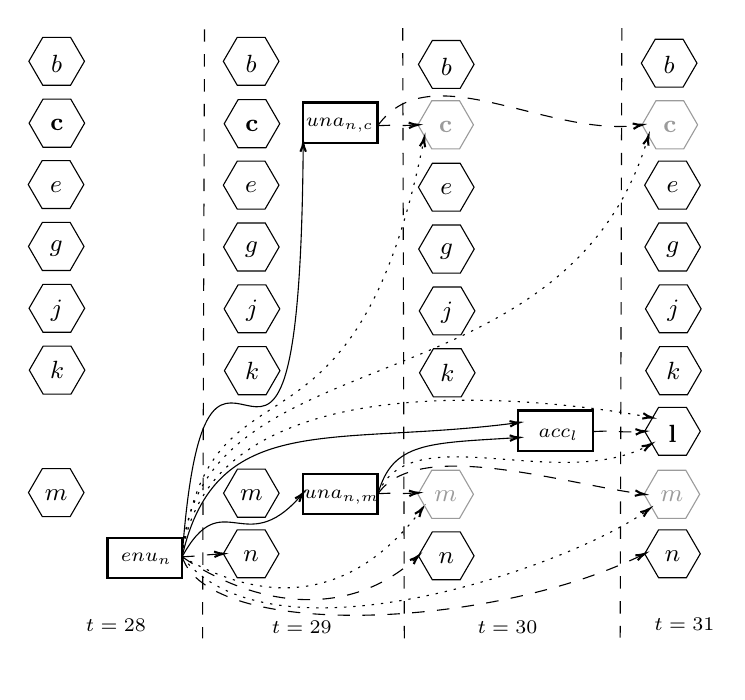
\begin{tikzpicture}[x=0.75pt,y=0.75pt,yscale=-1,xscale=1]
%uncomment if require: \path (0,300); %set diagram left start at 0, and has height of 300

%Shape: Rectangle [id:dp32394197299921523] 
\draw  [line width=0.75]  (38.8,251.2) -- (74.6,251.2) -- (74.6,270.54) -- (38.8,270.54) -- cycle ;
%Straight Lines [id:da5103454315814933] 
\draw  [dash pattern={on 4.5pt off 4.5pt}]  (85.53,6.3) -- (84.6,299.8) ;
%Straight Lines [id:da9625799604219181] 
\draw  [dash pattern={on 4.5pt off 4.5pt}]  (181.03,5.8) -- (181.8,299.8) ;
%Straight Lines [id:da937826652519754] 
\draw  [dash pattern={on 4.5pt off 4.5pt}]  (286.6,5.8) -- (285.8,299.4) ;
%Shape: Rectangle [id:dp39055029505322625] 
\draw  [line width=0.75]  (133.09,41.57) -- (168.89,41.57) -- (168.89,60.91) -- (133.09,60.91) -- cycle ;
%Shape: Polygon [id:dp25831662543105294] 
\draw   (27.7,21.73) -- (21,33.26) -- (7.6,33.26) -- (0.91,21.73) -- (7.6,10.19) -- (21,10.19) -- cycle ;
%Shape: Polygon [id:dp17264867524000027] 
\draw   (121.4,21.73) -- (114.7,33.26) -- (101.3,33.26) -- (94.6,21.73) -- (101.3,10.19) -- (114.7,10.19) -- cycle ;
%Shape: Polygon [id:dp9933858680624272] 
\draw   (215.4,23.23) -- (208.7,34.76) -- (195.3,34.76) -- (188.6,23.23) -- (195.3,11.69) -- (208.7,11.69) -- cycle ;
%Shape: Rectangle [id:dp8416513794122603] 
\draw  [line width=0.75]  (236.69,189.97) -- (272.49,189.97) -- (272.49,209.31) -- (236.69,209.31) -- cycle ;
%Curve Lines [id:da03689428077806867] 
\draw  [dash pattern={on 4.5pt off 4.5pt}]  (74.74,260.46) .. controls (110.24,284.75) and (154.9,290.88) .. (187.62,260.92) ;
\draw [shift={(188.6,260)}, rotate = 136.62] [color={rgb, 255:red, 0; green, 0; blue, 0 }  ][line width=0.75]    (4.37,-1.32) .. controls (2.78,-0.56) and (1.32,-0.12) .. (0,0) .. controls (1.32,0.12) and (2.78,0.56) .. (4.37,1.32)   ;
%Curve Lines [id:da9511759619364188] 
\draw    (74.74,260.46) .. controls (94.3,224.74) and (104.69,262.24) .. (131.75,231.26) ;
\draw [shift={(133,229.8)}, rotate = 129.81] [color={rgb, 255:red, 0; green, 0; blue, 0 }  ][line width=0.75]    (4.37,-1.32) .. controls (2.78,-0.56) and (1.32,-0.12) .. (0,0) .. controls (1.32,0.12) and (2.78,0.56) .. (4.37,1.32)   ;
%Shape: Regular Polygon [id:dp0962459706720944] 
\draw  [color={rgb, 255:red, 155; green, 155; blue, 155 }  ,draw opacity=1 ] (215.1,52.33) -- (208.41,63.92) -- (195.03,63.92) -- (188.34,52.33) -- (195.03,40.75) -- (208.41,40.75) -- cycle ;
%Curve Lines [id:da23781812589748064] 
\draw  [dash pattern={on 0.84pt off 2.51pt}]  (74.74,260.46) .. controls (136.15,295.88) and (173.1,260.09) .. (189.61,238.31) ;
\draw [shift={(190.6,237)}, rotate = 126.53] [color={rgb, 255:red, 0; green, 0; blue, 0 }  ][line width=0.75]    (4.37,-1.32) .. controls (2.78,-0.56) and (1.32,-0.12) .. (0,0) .. controls (1.32,0.12) and (2.78,0.56) .. (4.37,1.32)   ;
%Shape: Regular Polygon [id:dp5863365292722718] 
\draw   (27.78,51.53) -- (21.09,63.12) -- (7.71,63.12) -- (1.02,51.53) -- (7.71,39.95) -- (21.09,39.95) -- cycle ;
%Shape: Polygon [id:dp668166576601705] 
\draw   (27.4,81.13) -- (20.7,92.66) -- (7.3,92.66) -- (0.6,81.13) -- (7.3,69.59) -- (20.7,69.59) -- cycle ;
%Shape: Regular Polygon [id:dp1615790376024172] 
\draw   (27.48,110.93) -- (20.79,122.52) -- (7.41,122.52) -- (0.72,110.93) -- (7.41,99.35) -- (20.79,99.35) -- cycle ;
%Shape: Polygon [id:dp5652109778432169] 
\draw   (27.8,140.73) -- (21.1,152.26) -- (7.7,152.26) -- (1,140.73) -- (7.7,129.19) -- (21.1,129.19) -- cycle ;
%Shape: Regular Polygon [id:dp5554624960747061] 
\draw   (27.88,170.53) -- (21.19,182.12) -- (7.81,182.12) -- (1.12,170.53) -- (7.81,158.95) -- (21.19,158.95) -- cycle ;
%Shape: Regular Polygon [id:dp13320010668351145] 
\draw   (27.48,229.53) -- (20.79,241.12) -- (7.41,241.12) -- (0.72,229.53) -- (7.41,217.95) -- (20.79,217.95) -- cycle ;
%Shape: Regular Polygon [id:dp33133807114366276] 
\draw   (121.78,51.8) -- (115.09,63.39) -- (101.71,63.39) -- (95.02,51.8) -- (101.71,40.22) -- (115.09,40.22) -- cycle ;
%Shape: Polygon [id:dp7206917082119544] 
\draw   (121.4,81.4) -- (114.7,92.94) -- (101.3,92.94) -- (94.6,81.4) -- (101.3,69.86) -- (114.7,69.86) -- cycle ;
%Shape: Regular Polygon [id:dp689513993897114] 
\draw   (121.48,111.2) -- (114.79,122.79) -- (101.41,122.79) -- (94.72,111.2) -- (101.41,99.62) -- (114.79,99.62) -- cycle ;
%Shape: Polygon [id:dp3553082836345921] 
\draw   (121.8,141) -- (115.1,152.54) -- (101.7,152.54) -- (95,141) -- (101.7,129.46) -- (115.1,129.46) -- cycle ;
%Shape: Regular Polygon [id:dp08808706934177946] 
\draw   (121.88,170.8) -- (115.19,182.39) -- (101.81,182.39) -- (95.12,170.8) -- (101.81,159.22) -- (115.19,159.22) -- cycle ;
%Shape: Regular Polygon [id:dp3825724531298007] 
\draw   (121.48,229.8) -- (114.79,241.39) -- (101.41,241.39) -- (94.72,229.8) -- (101.41,218.22) -- (114.79,218.22) -- cycle ;
%Shape: Polygon [id:dp6015095613297166] 
\draw   (121.4,259) -- (114.7,270.54) -- (101.3,270.54) -- (94.6,259) -- (101.3,247.46) -- (114.7,247.46) -- cycle ;
%Shape: Polygon [id:dp9730868685192309] 
\draw   (215.4,82.4) -- (208.7,93.94) -- (195.3,93.94) -- (188.6,82.4) -- (195.3,70.86) -- (208.7,70.86) -- cycle ;
%Shape: Regular Polygon [id:dp04394747212171679] 
\draw   (215.48,112.2) -- (208.79,123.79) -- (195.41,123.79) -- (188.72,112.2) -- (195.41,100.62) -- (208.79,100.62) -- cycle ;
%Shape: Polygon [id:dp625486130912703] 
\draw   (215.8,142) -- (209.1,153.54) -- (195.7,153.54) -- (189,142) -- (195.7,130.46) -- (209.1,130.46) -- cycle ;
%Shape: Regular Polygon [id:dp6973070301209515] 
\draw   (215.88,171.8) -- (209.19,183.39) -- (195.81,183.39) -- (189.12,171.8) -- (195.81,160.22) -- (209.19,160.22) -- cycle ;
%Shape: Polygon [id:dp15730100429007365] 
\draw   (215.4,260) -- (208.7,271.54) -- (195.3,271.54) -- (188.6,260) -- (195.3,248.46) -- (208.7,248.46) -- cycle ;
%Shape: Polygon [id:dp7669928381847199] 
\draw   (324.4,81.4) -- (317.7,92.94) -- (304.3,92.94) -- (297.6,81.4) -- (304.3,69.86) -- (317.7,69.86) -- cycle ;
%Shape: Regular Polygon [id:dp8720689089102229] 
\draw   (324.48,111.2) -- (317.79,122.79) -- (304.41,122.79) -- (297.72,111.2) -- (304.41,99.62) -- (317.79,99.62) -- cycle ;
%Shape: Polygon [id:dp8686588781646976] 
\draw   (324.8,141) -- (318.1,152.54) -- (304.7,152.54) -- (298,141) -- (304.7,129.46) -- (318.1,129.46) -- cycle ;
%Shape: Regular Polygon [id:dp58257999600958] 
\draw   (324.88,170.8) -- (318.19,182.39) -- (304.81,182.39) -- (298.12,170.8) -- (304.81,159.22) -- (318.19,159.22) -- cycle ;
%Shape: Polygon [id:dp5246042913035425] 
\draw   (324.4,200) -- (317.7,211.54) -- (304.3,211.54) -- (297.6,200) -- (304.3,188.46) -- (317.7,188.46) -- cycle ;
%Shape: Polygon [id:dp40275693353577746] 
\draw   (324.4,259) -- (317.7,270.54) -- (304.3,270.54) -- (297.6,259) -- (304.3,247.46) -- (317.7,247.46) -- cycle ;
%Shape: Rectangle [id:dp294546304037402] 
\draw  [line width=0.75]  (133.09,220.57) -- (168.89,220.57) -- (168.89,239.91) -- (133.09,239.91) -- cycle ;
%Shape: Regular Polygon [id:dp13124017670187849] 
\draw  [color={rgb, 255:red, 155; green, 155; blue, 155 }  ,draw opacity=1 ] (323.1,52.33) -- (316.41,63.92) -- (303.03,63.92) -- (296.34,52.33) -- (303.03,40.75) -- (316.41,40.75) -- cycle ;
%Shape: Regular Polygon [id:dp6955758409780655] 
\draw  [color={rgb, 255:red, 155; green, 155; blue, 155 }  ,draw opacity=1 ] (215.1,230.33) -- (208.41,241.92) -- (195.03,241.92) -- (188.34,230.33) -- (195.03,218.75) -- (208.41,218.75) -- cycle ;
%Shape: Regular Polygon [id:dp41515587858602165] 
\draw  [color={rgb, 255:red, 155; green, 155; blue, 155 }  ,draw opacity=1 ] (324.1,230.33) -- (317.41,241.92) -- (304.03,241.92) -- (297.34,230.33) -- (304.03,218.75) -- (317.41,218.75) -- cycle ;
%Curve Lines [id:da9290568647401355] 
\draw    (74.74,260.46) .. controls (87.4,89) and (131.4,305) .. (133.09,60.91) ;
\draw [shift={(133.09,60.91)}, rotate = 90.4] [color={rgb, 255:red, 0; green, 0; blue, 0 }  ][line width=0.75]    (4.37,-1.32) .. controls (2.78,-0.56) and (1.32,-0.12) .. (0,0) .. controls (1.32,0.12) and (2.78,0.56) .. (4.37,1.32)   ;
%Curve Lines [id:da0024038948177537156] 
\draw    (74.74,260.46) .. controls (90.92,188.96) and (147.23,207.61) .. (235.66,195.98) ;
\draw [shift={(237,195.8)}, rotate = 172.34] [color={rgb, 255:red, 0; green, 0; blue, 0 }  ][line width=0.75]    (4.37,-1.32) .. controls (2.78,-0.56) and (1.32,-0.12) .. (0,0) .. controls (1.32,0.12) and (2.78,0.56) .. (4.37,1.32)   ;
%Curve Lines [id:da9423544130706317] 
\draw    (169.14,230.06) .. controls (176.09,204.98) and (193.66,205.77) .. (235.09,203.12) ;
\draw [shift={(237,203)}, rotate = 176.26] [color={rgb, 255:red, 0; green, 0; blue, 0 }  ][line width=0.75]    (4.37,-1.32) .. controls (2.78,-0.56) and (1.32,-0.12) .. (0,0) .. controls (1.32,0.12) and (2.78,0.56) .. (4.37,1.32)   ;
%Curve Lines [id:da07687685155568191] 
\draw  [dash pattern={on 4.5pt off 4.5pt}]  (74.74,260.46) .. controls (88.13,300.8) and (222.84,295.45) .. (296.5,259.54) ;
\draw [shift={(297.6,259)}, rotate = 153.62] [color={rgb, 255:red, 0; green, 0; blue, 0 }  ][line width=0.75]    (4.37,-1.32) .. controls (2.78,-0.56) and (1.32,-0.12) .. (0,0) .. controls (1.32,0.12) and (2.78,0.56) .. (4.37,1.32)   ;
%Curve Lines [id:da17080960388415456] 
\draw  [dash pattern={on 4.5pt off 4.5pt}]  (74.74,260.46) .. controls (88.36,259.78) and (80.46,259.9) .. (92.73,259.12) ;
\draw [shift={(94.6,259)}, rotate = 176.49] [color={rgb, 255:red, 0; green, 0; blue, 0 }  ][line width=0.75]    (4.37,-1.32) .. controls (2.78,-0.56) and (1.32,-0.12) .. (0,0) .. controls (1.32,0.12) and (2.78,0.56) .. (4.37,1.32)   ;
%Curve Lines [id:da6369256315030506] 
\draw  [dash pattern={on 4.5pt off 4.5pt}]  (169,52.78) .. controls (182.62,52.1) and (174.24,53.15) .. (186.47,52.44) ;
\draw [shift={(188.34,52.33)}, rotate = 176.49] [color={rgb, 255:red, 0; green, 0; blue, 0 }  ][line width=0.75]    (4.37,-1.32) .. controls (2.78,-0.56) and (1.32,-0.12) .. (0,0) .. controls (1.32,0.12) and (2.78,0.56) .. (4.37,1.32)   ;
%Curve Lines [id:da5460890529535121] 
\draw  [dash pattern={on 4.5pt off 4.5pt}]  (169.14,230.06) .. controls (182.76,229.38) and (174.38,230.43) .. (186.61,229.73) ;
\draw [shift={(188.48,229.62)}, rotate = 176.49] [color={rgb, 255:red, 0; green, 0; blue, 0 }  ][line width=0.75]    (4.37,-1.32) .. controls (2.78,-0.56) and (1.32,-0.12) .. (0,0) .. controls (1.32,0.12) and (2.78,0.56) .. (4.37,1.32)   ;
%Curve Lines [id:da9866128326016497] 
\draw  [dash pattern={on 4.5pt off 4.5pt}]  (169.14,230.06) .. controls (187.91,203.01) and (256.5,224.73) .. (295.58,230.1) ;
\draw [shift={(297.34,230.33)}, rotate = 187.26] [color={rgb, 255:red, 0; green, 0; blue, 0 }  ][line width=0.75]    (4.37,-1.32) .. controls (2.78,-0.56) and (1.32,-0.12) .. (0,0) .. controls (1.32,0.12) and (2.78,0.56) .. (4.37,1.32)   ;
%Curve Lines [id:da3372282256776671] 
\draw  [dash pattern={on 4.5pt off 4.5pt}]  (169,52.78) .. controls (193.95,17.75) and (250.26,58.57) .. (294.99,52.53) ;
\draw [shift={(296.34,52.33)}, rotate = 171.06] [color={rgb, 255:red, 0; green, 0; blue, 0 }  ][line width=0.75]    (4.37,-1.32) .. controls (2.78,-0.56) and (1.32,-0.12) .. (0,0) .. controls (1.32,0.12) and (2.78,0.56) .. (4.37,1.32)   ;
%Curve Lines [id:da7931620072938754] 
\draw  [dash pattern={on 4.5pt off 4.5pt}]  (273.22,200.11) .. controls (286.84,199.43) and (283.06,200.78) .. (295.7,200.11) ;
\draw [shift={(297.6,200)}, rotate = 176.49] [color={rgb, 255:red, 0; green, 0; blue, 0 }  ][line width=0.75]    (4.37,-1.32) .. controls (2.78,-0.56) and (1.32,-0.12) .. (0,0) .. controls (1.32,0.12) and (2.78,0.56) .. (4.37,1.32)   ;
%Curve Lines [id:da3170103066051301] 
\draw  [dash pattern={on 0.84pt off 2.51pt}]  (74.74,260.46) .. controls (118.16,315.64) and (262.47,264.45) .. (298.73,238.19) ;
\draw [shift={(299.8,237.4)}, rotate = 142.92] [color={rgb, 255:red, 0; green, 0; blue, 0 }  ][line width=0.75]    (4.37,-1.32) .. controls (2.78,-0.56) and (1.32,-0.12) .. (0,0) .. controls (1.32,0.12) and (2.78,0.56) .. (4.37,1.32)   ;
%Curve Lines [id:da2974445519606693] 
\draw  [dash pattern={on 0.84pt off 2.51pt}]  (74.74,260.46) .. controls (87.54,158.68) and (268.35,187.37) .. (299.3,193.08) ;
\draw [shift={(301,193.4)}, rotate = 190.78] [color={rgb, 255:red, 0; green, 0; blue, 0 }  ][line width=0.75]    (4.37,-1.32) .. controls (2.78,-0.56) and (1.32,-0.12) .. (0,0) .. controls (1.32,0.12) and (2.78,0.56) .. (4.37,1.32)   ;
%Curve Lines [id:da007173676928789563] 
\draw  [dash pattern={on 0.84pt off 2.51pt}]  (74.74,260.46) .. controls (87.8,155) and (157.8,229.8) .. (191.4,58.6) ;
\draw [shift={(191.4,58.6)}, rotate = 101.1] [color={rgb, 255:red, 0; green, 0; blue, 0 }  ][line width=0.75]    (4.37,-1.32) .. controls (2.78,-0.56) and (1.32,-0.12) .. (0,0) .. controls (1.32,0.12) and (2.78,0.56) .. (4.37,1.32)   ;
%Curve Lines [id:da8424571147503932] 
\draw  [dash pattern={on 0.84pt off 2.51pt}]  (74.74,260.46) .. controls (81.4,151.4) and (260.2,192.6) .. (299.4,57.8) ;
\draw [shift={(299.4,57.8)}, rotate = 106.21] [color={rgb, 255:red, 0; green, 0; blue, 0 }  ][line width=0.75]    (4.37,-1.32) .. controls (2.78,-0.56) and (1.32,-0.12) .. (0,0) .. controls (1.32,0.12) and (2.78,0.56) .. (4.37,1.32)   ;
%Curve Lines [id:da832051990599513] 
\draw  [dash pattern={on 0.84pt off 2.51pt}]  (169.14,230.06) .. controls (184.45,192.58) and (255.95,229.84) .. (299.3,206.91) ;
\draw [shift={(300.6,206.2)}, rotate = 150.54] [color={rgb, 255:red, 0; green, 0; blue, 0 }  ][line width=0.75]    (4.37,-1.32) .. controls (2.78,-0.56) and (1.32,-0.12) .. (0,0) .. controls (1.32,0.12) and (2.78,0.56) .. (4.37,1.32)   ;
%Shape: Polygon [id:dp822443066516893] 
\draw   (322.8,22.63) -- (316.1,34.16) -- (302.7,34.16) -- (296,22.63) -- (302.7,11.09) -- (316.1,11.09) -- cycle ;

% Text Node
\draw (27.13,289.4) node [anchor=north west][inner sep=0.75pt]  [font=\scriptsize]  {$t=28$};
% Text Node
\draw (44,257.6) node [anchor=north west][inner sep=0.75pt]  [font=\scriptsize]  {$enu_{n}$};
% Text Node
\draw (133.09,47.97) node [anchor=north west][inner sep=0.75pt]  [font=\scriptsize]  {$una_{n,c}$};
% Text Node
\draw (116.67,290.33) node [anchor=north west][inner sep=0.75pt]  [font=\scriptsize]  {$t=29$};
% Text Node
\draw (215.8,289.9) node [anchor=north west][inner sep=0.75pt]  [font=\scriptsize]  {$t=30$};
% Text Node
\draw (301,288.9) node [anchor=north west][inner sep=0.75pt]  [font=\scriptsize]  {$t=31$};
% Text Node
\draw (14.3,22.73) node  [font=\small]  {$b$};
% Text Node
\draw (108,22.73) node  [font=\small]  {$b$};
% Text Node
\draw (202,24.23) node  [font=\small]  {$b$};
% Text Node
\draw (245.19,197.57) node [anchor=north west][inner sep=0.75pt]  [font=\scriptsize]  {$acc_{l}$};
% Text Node
\draw (201.72,53.33) node  [font=\small,color={rgb, 255:red, 155; green, 155; blue, 155 }  ,opacity=1 ]  {$\mathbf{c}$};
% Text Node
\draw (14.4,52.53) node  [font=\small]  {$\mathbf{c}$};
% Text Node
\draw (14,82.13) node  [font=\small]  {$e$};
% Text Node
\draw (14.1,111.93) node  [font=\small]  {$g$};
% Text Node
\draw (14.4,141.73) node  [font=\small]  {$j$};
% Text Node
\draw (14.5,170.53) node  [font=\small]  {$k$};
% Text Node
\draw (14.1,230.53) node  [font=\small]  {$m$};
% Text Node
\draw (108.4,52.8) node  [font=\small]  {$\mathbf{c}$};
% Text Node
\draw (108,82.4) node  [font=\small]  {$e$};
% Text Node
\draw (108.1,112.2) node  [font=\small]  {$g$};
% Text Node
\draw (108.4,142) node  [font=\small]  {$j$};
% Text Node
\draw (108.5,170.8) node  [font=\small]  {$k$};
% Text Node
\draw (108.1,230.8) node  [font=\small]  {$m$};
% Text Node
\draw (108,260) node  [font=\small]  {$n$};
% Text Node
\draw (202,83.4) node  [font=\small]  {$e$};
% Text Node
\draw (202.1,113.2) node  [font=\small]  {$g$};
% Text Node
\draw (202.4,143) node  [font=\small]  {$j$};
% Text Node
\draw (202.5,171.8) node  [font=\small]  {$k$};
% Text Node
\draw (202,261) node  [font=\small]  {$n$};
% Text Node
\draw (311,82.4) node  [font=\small]  {$e$};
% Text Node
\draw (311.1,112.2) node  [font=\small]  {$g$};
% Text Node
\draw (311.4,142) node  [font=\small]  {$j$};
% Text Node
\draw (311.5,170.8) node  [font=\small]  {$k$};
% Text Node
\draw (311,201) node  [font=\small]  {$\mathbf{l}$};
% Text Node
\draw (311,260) node  [font=\small]  {$n$};
% Text Node
\draw (132.09,226.97) node [anchor=north west][inner sep=0.75pt]  [font=\scriptsize]  {$una_{n,m}$};
% Text Node
\draw (309.72,53.33) node  [font=\small,color={rgb, 255:red, 155; green, 155; blue, 155 }  ,opacity=1 ]  {$\mathbf{c}$};
% Text Node
\draw (201.72,231.33) node  [font=\small,color={rgb, 255:red, 155; green, 155; blue, 155 }  ,opacity=1 ]  {$m$};
% Text Node
\draw (310.72,231.33) node  [font=\small,color={rgb, 255:red, 155; green, 155; blue, 155 }  ,opacity=1 ]  {$m$};
% Text Node
\draw (309.4,23.63) node  [font=\small]  {$b$};


\end{tikzpicture}
}
        	\caption{Enriched graphical representation of Example~\ref{ex:IRM_ou_radio}, with causal relations extracts:  Direct NESS-causes \DirectNESS, NESS-causes \NESS, and actual causes \actual.}
        	\label{fig:exemple_fin}
        \end{figure}
        
        \addtocounter{example}{-2}
        \begin{example} (continued) --
            %Since the representation of the traces of events and states is the same as in Figure~\ref{fig:exemple_ini}, we only comment on the causal relations found in Figure~\ref{fig:exemple_fin}. Recall that arguments~$a$, $c$ and~$l$ are the decision variables. As argument~$a$ becomes unacceptable very early in the dialogue and remains so throughout, we have chosen not to represent it in the figures.
 Figure~\ref{fig:exemple_fin} graphically displays 
%  the for
 the last four states in the trace of  Example~\ref{ex:IRM_ou_radio},  corresponding to the enunciation of argument~$n$ and the subsequent update mechanisms.           
Argument~$n$, which states the urgency of the examination,
is the one that closes the debate. As represented in Figure~\ref{fig:exemple_fin}  its enunciation in state~$S(28)$ is a direct NESS-cause (dNc) of its acceptability in the following states, a relation we denote by~$(enunciate_n,28)$ dNc $(a_n,29-31)$. Similarly, we have $(makesUnacc_{n,c},29)$ dNc $(\neg a_c,{30-31})$, $(makesUnacc_{n,m},29)$ dNc ${(\neg a_m,30-31)}$, and $(makesAcc_l,30)$ dNc $(a_l,31)$. As these examples show, this first relationship is the basic building block of causality, which is concerned with causal relationships given the actual effects of the occurrence of an event. Yet this relationship is not enough. If we want to know why argument~$l$  is acceptable at the end of the dialogue (i.e. why the decision to have an MRI on the same day is made), it is not satisfactory to simply say that it is because of the event~$(makesAcc_l,30)$.
           
To find out why the latter happens, we need to look at the NESS causes and the actual causes to construct the causal chain that lead to it. By transitivity we get that $(makesUnacc_{n,m},29)$ is a cause of the fact that $makesAcc_l$ was triggered, and therefore of the effects that triggering may have had. Going back even further and looking for the causes for which the occurrence~$(makesUnacc_{n,m},29)$ took place, we find $(enunciate_n,28)$ actual cause~$(makesUnacc_{n,m},29)$ and therefore $(enunciate_n,28)$ NESS-cause~$(\neg a_m,30-31)$. By transitivity we can derive $(enunciate_n,28)$ NESS-cause~$(a_l,31)$. This new relation allows us to say that the physician enunciating that it is an emergency is one of the causes of the final decision, an answer that already seems more satisfactory and can be included in an explanation. The same reasoning can be applied to find the causes of $(\neg a_c,31)$, the other decision variable.
        \end{example}
    

        % For these reasons, in our approach we propose for the moment only a visual representation of the mechanism leading to the decision. They can obviously be a support for an explanation but do not provide one independently. To be able to provide one, 
        % The latter has the advantage of making it possible to represent the whole causal chain thanks to figures like the one presented in Figure~\ref{fig:exemple_fin}. 
        % If we wish to be interested in the generation of textual explanations adapted to humans, we will have to start by defining what an explanation is in this formalism, including in particular a notion of contrast within the explanation. It will also be important to determine how and which causes to choose for the explanation.
        % \Isa{on pourrait peut-être raccourcir cette fin, en notant juste ce qu'il faudrait ajouter pour arriver à des explications simples, minimales, contrastives, etc. (et c'est déjà un peu dit dans les perspectives plus loin)}